\section{Stable Diffusion}
\label{sec:stable_diffusion}

\begin{figure}
    \centering
    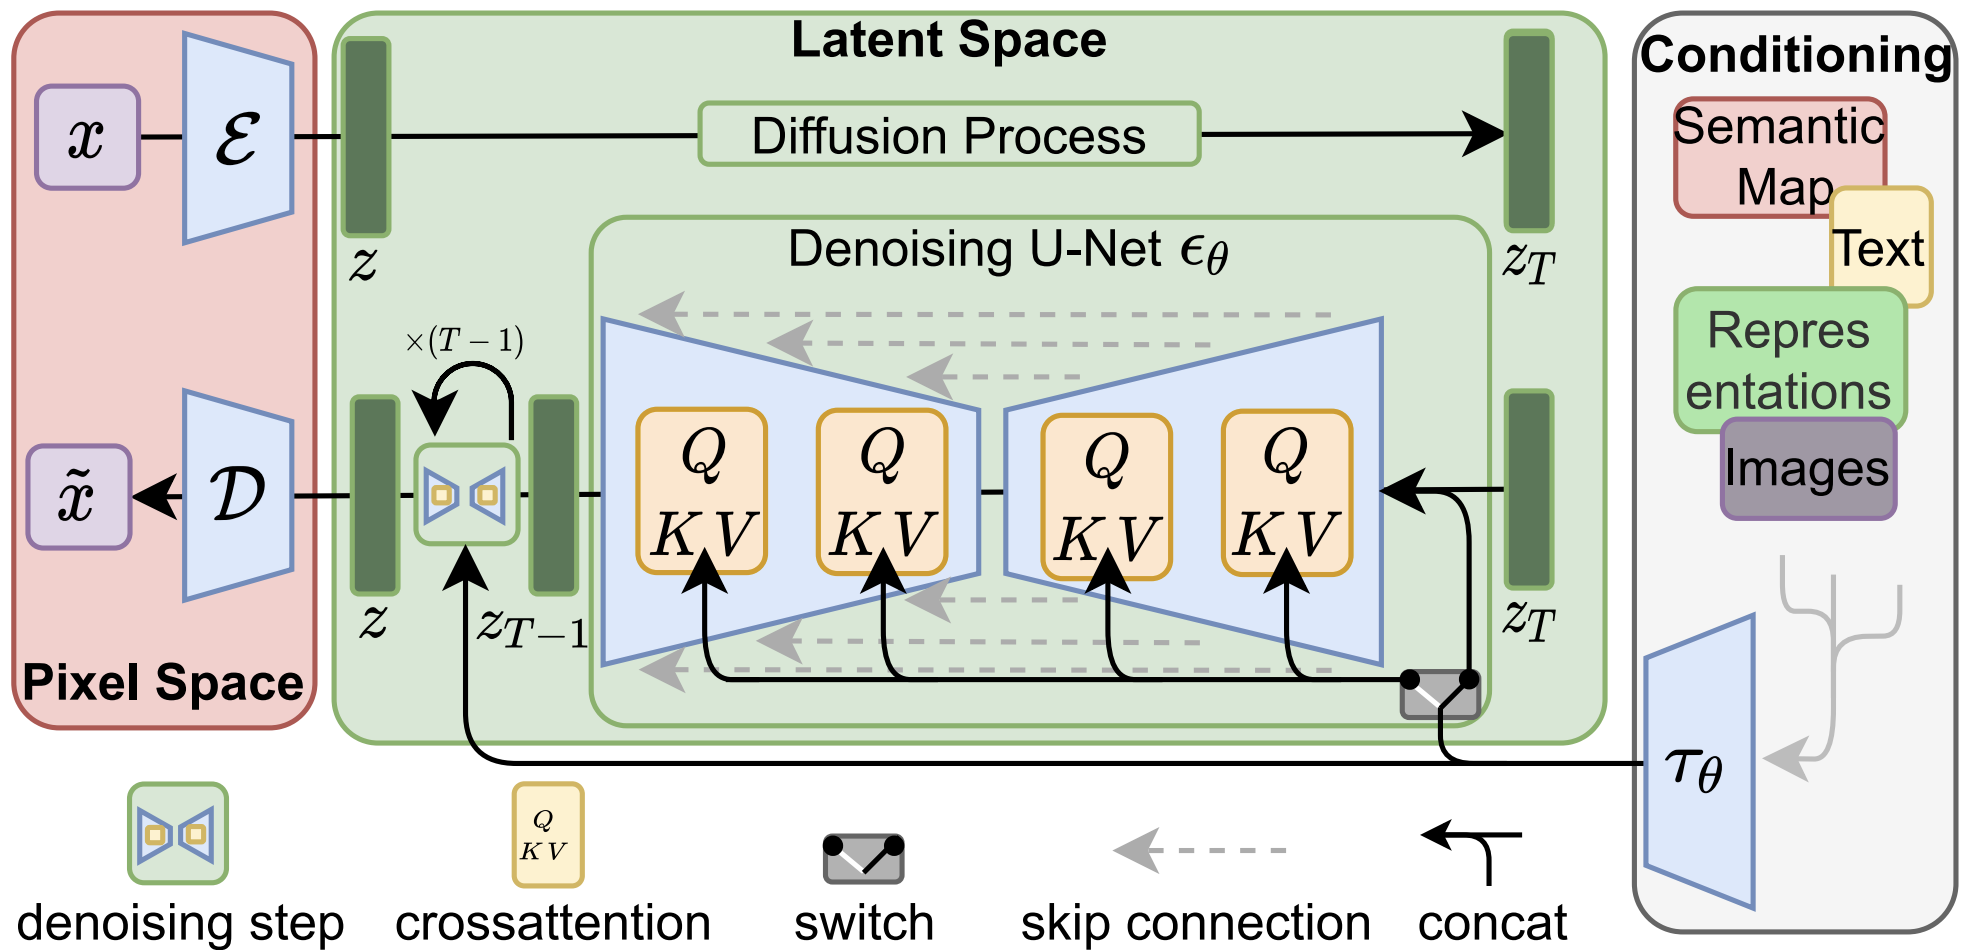
\includegraphics[width=1\textwidth]{images/diffusion_models/stable_diffusion.png}
    \caption{Stable diffusion process in Stable Diffusion Models (SDMs) \cite{stable_diffusion}.}
    \label{fig:stable_diffusion}
\end{figure}

Stable diffusion models are based on latent diffusion. In the paper \cite{stable_diffusion} the authors suggested that computing gradients directly on RGB space is inefficient, since this space is high-dimentional. Instead, they suggest to first convert the training images to a lower-dimensional latent space and then apply the diffusion processes on this space.

This process is much more efficient, and in the paper \cite{stable_diffusion} the authors showed that the model can be trained on a single GPU with 16GB of memory. The model is trained on a 256x256 resolution CelebA-HQ dataset with 30 diffusion steps.

An example of this is when giving an image to a person and asking them to describe the image, they will not describe the individual pixel values, but instead describe the high-level features of the image first.

A 2021 paper released by OpenAI \cite{openai_diffusion_beats_gans} shows that diffusion models can outperform GANs in terms of image fidelity by trading off diversity.








\subsection{Classifier-free diffusion guidance}

\label{subsec:classifier_free_diffusion_guidance}

Conditioning a generative model can be done in many ways. How can we let our model understand our text prompt? Or condition on another image? One way is to train a model to learn a joint distribution of the training data and the conditioning signal $p(x,c)$ and then sample from the joint distribution. This, however, requires the training of a model for each seperate conditioning signal.

Another approach is called \textbf{classifier guidance} \cite{openai_diffusion_beats_gans} which involves the training of a seperate model to condition the output. The latest and most successful approach is called \textbf{classifier-free guidance} \cite{classifier_free_guidance}, in which, instead of training two networks, one conditional network and an unconditional network, we train a single network and during training, with some probability, we set the conditioning signal to zero. This way the network becomes a mix of conditined and unconditioned network, and we can take the conditioned and unconditioned output and combine them with weight that indicates how much we want the network to pay attention to the conditioning signal.






\subsection{Contrastive Language-Image Pre-training (CLIP)}

\label{subsec:clip}







\subsection{Training}

Stable diffusion uses two-stage approach, called classifier-free guidance (see \ref{subsec:classifier_free_diffusion_guidance}) which was discuessed before. 